% -*- coding: utf-8 -*-

\begin{chapter}{Уравнение Движения}\label{chap:7}
% \chapter[The Equations of Motion]{Some Mathematics: The Equations of Motion}
В этой главе мы рассмотрим как реагирует поток на внешние и внутренние
силы.  Это приведёт к выводу некоторых основных уравнений описывающих
динамику океана. В следующей главе мы обсудим влияние трения а в
главе~12 последствия завихренности.
%
% In this chapter I consider the response of a fluid to internal and external
% forces. This leads to a derivation of some of the basic equations describing
% ocean dynamics. In the next chapter, we will consider the influence
% of viscosity, and in chapter 12 we will consider the consequences
% of vorticity.

Гидромеханика использующаяся в океанографии основана на Ньютоновской
динамике, модифицированной в свете наших представлений о
турбулентности. Законы сохранения массы, импульса, количества движения
и энергии приводят к формулам с названиями скрывающими их
происхождение.  
%
% Fluid mechanics used in oceanography is based on Newtonian mechanics 
% modified by our evolving understanding of turbulence\index{turbulence}.
% Conservation of mass, momentum, angular momentum, and energy lead to
% particular equations having names that hide their origins (table 7.1).

\begin{table}
\caption{Законы Сохранения приводящие к основным уравнениям движения жидкости}
\begin{tabular}{ll}
Закон Сохранения Массы:
 & Приводит к Уравнению Неразрывности.\\
Закон Сохранения Энергии
 & Закон Сохранения Тепла приводит к Уравнению Теплового Баланса. 
   Закон Сохранения Механической Энергии приводит к Волновому Уравнению.\\
Закон Сохранения Импульса:
 & Приводит к Уравнению Количества Движения (Навье-Стокса).\\
Закон Сохранения Углового Момента:
& Приводит к Закону Сохранения Вихря.\\
\end{tabular}
\end{table}
%
% \begin{table}[h!] \small
% \vspace{-1ex}
% \begin{tabular*}{121mm}{@{}ll@{}}
% \multicolumn{2} {@{}l@{}}{\bfseries Table 7.1 Conservation Laws
% \index{conservation laws}Leading to
% Basic\rule[-1ex]{0mm}{1ex} Equations of Fluid Motion} \\
% \hline
% \rule{0ex}{2.5ex}Conservation of Mass: & Leads to Continuity Equation. \\
% Conservation of Energy: & Conservation of heat leads to Heat Budgets. \\
%  & Conservation of mechanical energy leads to \\
%  & \hspace{1em}Wave Equation. \\
% Conservation of Momentum:& Leads to Momentum (Navier-Stokes) Eq. \\
% Conservation of Angular Momentum: & Leads to Conservation of Vorticity. \\
% \hline
% \end{tabular*} \\[0.5ex]
% \vspace{-3ex}
% \end{table}

\begin{section}{Основные силы в океане}
% \section{Dominant Forces for Ocean Dynamics}
Всего несколько сил важны для физической океанографии: сила тяжести,
сила плавучести (в результате различной плотности морской воды) и
напряжения ветра. Помните что силы~--- это вектора. Они имеют
величину и направление.
%
% \index{ocean!dominant forces in}Only a few forces are important in 
% physical oceanography: gravity, friction, and Coriolis (table 7.2).
% Remember that forces are vectors. They have magnitude and direction.
%
\begin{enumerate}
\item
\textbf{Сила Тяжести}~--- основная сила. Столб воды в океане создаёт
давление, а изменения высоты столба воды создают горизонтальный
градиент давления. Изменения силы тяжести вследствии движения Солнца и
Луны относительно Земли вызывают приливы, приливные течения и
приливное перемешивание в толще океана.
%
% \vitem \textit{Gravity} \index{gravity|textbf}is the dominant force. 
% The weight of the water in the ocean produces pressure. Changes in gravity,
% due to the motion of sun\index{sun} and moon\index{moon} relative
% to earth produces tides, tidal currents, and tidal
% mixing\index{mixing!tidal} in the interior of the ocean.

\item
\textbf{Сила Плавучести} (архимедова сила)~--- сила направленная вверх
или вниз, действующая на (единичную)массу жидкости более плотную или
менее плотную чем окружающая вода. Например холодный ветер дующий над
морем охлаждает поверхностную воду делая её более плотной чем
нижележащая вода. Различия в плотности вызывают силу заставляющую
поверхностную воду опускаться.
%
% \textit{Buoyancy} \index{buoyancy|textbf}is the upward or downward force 
% due to gravity acting on a parcel of water that is more or less dense
% than other water at its level. For example, cold air blowing over
% the sea cools surface waters causing them to be more dense than the water
% beneath. Gravity acting on the difference in density results in a
% force that causes the water to sink. 

% \textit{Horizontal pressure gradients} 
% \index{pressure gradient!horizontal|textbf}are due to the varying weight
% of water in different regions of the ocean. 
%
% \vitem \textit{Friction} \index{friction|textbf}is the force acting 
% on a body as it moves past another body while in contact with that body.
% The bodies can be parcels of water or air.

\item
\textbf{Ветер} дующий над поверхностью моря передаёт ему
горизонтальный импульс. Он тащит воду в направлении своего действия и
создаёт турбулентность перемешивающую верхнии слои воды, в результате
появляется океанический слой перемешивания. Кроме того ветер дующий
над морской рябью приводит к необычному (особому) распределению
давления над ней и заставляет рябь вырастать в волны.
%
% \textit{Wind stress} \index{wind|textbf}is the friction due to wind 
% blowing across the sea surface. It transfers horizontal momentum to the sea,
% creating currents. Wind blowing over waves on the sea surface leads 
% to an uneven distribution of pressure over the waves. The pressure 
% distribution transfers energy to the waves, causing them to grow into
% bigger waves.

\item
\textbf{Псевдо-силы}~--- мнимые силы которые возникают при
криволинейном движении или вращении системы координат. Таким образом в
уравнениях движения для вращающейся системы координат появляются
дополнительные члены, называющиеся псевдо силами. Например первый
закон Ньютона утверждает что движение тела не изменится пока на него
не подействует сила. Тем не менее во вращающейся системе координат
будет казаться что тело движущееся с постоянной скоростью изменяет
направление. Изменение направления приписывается псевдо силе~--- Силе
Кориолиса.
%
% \vitem\textit{Pseudo-forces} \index{pseudo-forces|textbf}are apparent 
% forces that arise from motion in curvilinear or rotating coordinate systems.
% For example, Newton's first law states that there is no change in motion
% of a body unless a resultant force acts on it. Yet a body moving at
% constant velocity seems to change direction when viewed from a rotating
% coordinate system. The change in direction is due to a pseudo-force,
% the Coriolis force.

\item
\textbf{Сила Кориолиса}~--- основная псевдо сила влияющая на
перемещение течений в системе координат связанной с Землёй.
%
% \textit{Coriolis Force} \index{Coriolis force|textbf}is the dominant
% pseudo-force influencing motion in a coordinate system fixed to the earth.
\end{enumerate}

\begin{table}
\caption{Силы в геофизической Гидродинамике.}
\begin{tabular}{ll}
\textbf{Основные силы} \\
Тяжести&Источник сил давления и приливов.\\
Действия Ветра&Вызывает движения на поверхности океана\\
Плавучести&Возникает из за разницы в плотности, приводит к конвекции.\\
\textbf{Другие Силы} \\
Атмосферного давления&Вызывает эффект обратного барометра.\\
Сейсмические&Вызывают цунами в результате землятрясений.\\
\end{tabular}
Обратите внимание что последние две силы важны гораздо меньше чем первые три.
\end{table}
%
% \begin{table}[h!] \small{{\textbf{Table 7.2 Forces in Geophysical Fluid Dynamics}}
% \\[1ex]
% \vspace{-6ex}
% \begin{tabular*}{121mm}{@{}ll@{}}
% \hline
% \textbf{Dominant Forces}\rule{0pt}{2.5ex}    & \\
% Gravity                                   & Gives rise to pressure gradients, buoyancy, and  tides. \\
% Coriolis                                  & Results from motion in a rotating coordinate system \\
% Friction                                  & Is due to relative motion between two fluid parcels. \\
%                                                 & Wind stress is an important frictional force. \\
% \textbf{Other Forces}            & \rule{0mm}{4.5ex}\\
% Atmospheric Pressure        & Results in inverted barometer effect. \\
% Seismic                                  & Results in \textit{tsunamis} driven by earthquakes. \\ [0.5ex]
% \hline
% \multicolumn{2}{@{}l@{}}{Note\rule{0mm}{2.5ex} that the last two forces are much less important than the first three.} \\
% \end{tabular*} \\ [0.5ex]}
% \rule{0ex}{2ex}
% %\vspace{-3ex}
% \end{table}
\end{section}

\begin{section}{Система координат}
% \section{Coordinate System}
Система координат позволяет нам определять положение при теоритических
и практических исследованиях. В зависимости от размеров элементов
которые нужно описать или картировать используют разные системы
координат. Я кратко расскажу о самых простейших системах; описание
более сложных можно найти в географических и геодезических книгах.
%
% \index{coordinate systems}Coordinate systems allow us to find
% locations in theory and practice. Various systems are used
% depending on the size of the features to be described or mapped. I
% will refer to the simplest systems; descriptions of other systems
% can be found in geography and geodesy books.

\begin{enumerate}
\item
\textbf{Декартова (прямоугольная) система координат}~--- её я буду
использовать наиболее часто в последующих главах. Она делает описание
настолько простым насколько это вообще возможно. В декартовой системе
мы можем описать большинство процессов без математических сложностей
присущих сферической системе. По традиции в геофизической
гидромехинике ось~$x$ направлена на восток, ось~$y$ на север, а
ось~$z$ вверх.
%
% \vitem\textit{Cartesian Coordinate System} \index{coordinate 
% systems!Cartesian|textbf}is the one I will use most commonly in the 
% following chapters to keep the discussion as simple as possible. We can
% describe most processes in Cartesian coordinates without the mathematical
% complexity of spherical coordinates. The standard convention in geophysical
% fluid mechanics is $x$ is to the east, $y$ is to the north, and $z$ is up. 

\item
\textbf{f-плоскость.} Это Прямоугольная система координат в которой
сила Кориолиса считается постоянной. Она используется при описании
потоков в районах мало сравнимых с радиусом Земли и с характерными
масштабами больше нескольких десятков километров.
%
% \textit{f-Plane}
% \index{coordinate systems!f-plane|textbf}\index{f-plane@\textit{f}-plane|textbf}is
% a Cartesian coordinate system in which the Coriolis force is assumed
% constant. It is useful for describing flow in regions small compared with
% the radius of the earth and larger than a few tens of kilometers. 

\item
\textbf{b-плоскость.} Прямоугольная система координат в которой сила
Кориолиса принимается линейно изменяющейся с широтой. Она используется
для описания потоков в масштабах океанических бассейнов.
%
% \textit{$\beta$-plane}
% \index{coordinate 
% systems!B-plane@$\beta$-plane|textbf}\index{B-plane@$\beta$-plane|textbf}is
% a Cartesian coordinate system in which the Coriolis force is assumed to
% vary linearly with latitude. It is useful for describing flow over areas
% as large as ocean basins.

\item
\textbf{Сферические координаты} 
иногда используются в численных моделях бассейнов и течений глобального 
масштаба для описания потоков прострирающихся на большие расстояния.
%
% \vitem\textit{Spherical coordinates} \index{coordinate systems!spherical coordinates|textbf}are 
% used to describe flows that extend over large distances and in numerical 
% calculations of basin and global scale flows.
\end{enumerate}
\end{section}

\begin{section}{Типы потоков в океане}
% \section{Types of Flow in the ocean}
Существует много способов описания циркуляции океана. Вот некоторые
широко распространённые термины для течений и волн.
%
% \index{flow!types of}Many terms are used for describing the ocean
% circulation. Here are a few of the more commonly used terms for
% describing currents and waves.

\begin{enumerate}
\item
\textbf{Общая Циркуляция}~--- это постоянная, усреднённая по времени
циркуляция океана.
%
% \vitem\textit{General Circulation} \index{general circulation|textbf}is
% the permanent, time-averaged circulation.

\item
\textbf{Меридиональная} (противоциркуляция, обратная циркуляция) также
известная как Термохалинная Циркуляция~--- циркуляция в меридиональной
плоскости, вызванная разницей плотности.
%
% \vitem\textit{Abyssal} \index{abyssal circulation|textbf}also called the
% \textit{Deep Circulation} \index{deep circulation|textbf}is
% the circulation of mass, in the meridional plane, in the deep ocean, 
% driven by mixing.

\item
\textbf{Ветровая Циркуляция}~--- циркуляция в верхнем километровом
слое океана, она может образоваваться как за счёт локальных ветров,
так и ветров дующих над большими регионами.
%
% \vitem\textit{Wind-Driven Circulation} \index{wind-driven circulation|textbf}is the
% circulation in the upper kilometer of the ocean forced by the wind. 
% The circulation can be caused by local winds or by winds in other regions. 

\item
\textbf{(кольца)} ветровые циклонически и антициклонически
направленные системы течений, с характерными масштабами сравнимыми с
размерами океанических бассейнов.
%
% \vitem\textit{Gyres}\index{gyres|textbf} are wind-driven cyclonic or 
% anticyclonic currents with dimensions nearly that of ocean basins.

\item
\textbf{Вдольбереговые Течения}~--- течения текущие паралельно
побережью. Важны два их типа: 
%
% \vitem\textit{Boundary Currents} \index{boundary currents|textbf}are currents
% flowing parallel to coasts. Two types of boundary currents are important:
%
\begin{itemize}
 \item западные вдольбереговые течения располагаются на западной
 границе океанов и представляют собой быстрые узкие струи, такие как
 Куросио и Гольфстрим.
%
% \vitem Western boundary currents on the western edge of the ocean tend to be
% fast, narrow jets such as the Gulf Stream\index{Gulf Stream!as a western 
% boundary current} and Kuroshio\index{Kuroshio!as a western boundary current}.

 \item восточные вдольбереговые течения слабые, например Калифорнийское
 течение.
%
% \vitem Eastern boundary currents are weak, \textit{e.g}. the California
% Current.
\end{itemize}

\item
\textbf{Струйные Течения}~--- протяжённые узкие течения, с
пространственными размерами в несколько сотен километров, почти
перпендикулярные западному побережью.
%
% \vitem\textit{Squirts} \index{squirts|textbf}or \textit{Jets}
% \index{jets|textbf}are long narrow currents, with dimensions of a few hundred
% kilometers, that are nearly perpendicular to west coasts. 

\item
\textbf{Среднемасштабные вихревые потоки} или волны похожие на течения
с масштабами в несколько сот километров.
%
% \vitem\textit{Mesoscale Eddies}
% \index{mesoscale eddies|textbf}are turbulent or spinning flows on scales 
% of a few hundred kilometers.

\item
\textbf{Штормовые Нагоны}~--- изменения уровня моря вызванное штормами
приходящими на побережья с широким и мелким континентальным шельфом,
такие как Мексиканский Залив и Северное море.
\end{enumerate}

Кроме потоков вызванных течениями существует много типов колебательных
(неустойчивывх) потоков вызванных волнами. Обычно когда мы думаем о
волнах в море мы представляем себе волны разбивающиеся о берег или
качающие морские корабли. Но в океане существуют и другие виды волн.
%
% In addition to flow due to currents, there are many types of oscillatory 
% flows due to waves. Normally, when we think of waves in the ocean,
% we visualize waves breaking on the beach or the surface waves influencing
% ships at sea. But many other types of waves occur in the ocean.
%
\begin{enumerate}
\item
\textbf{Планетарные Волны} зависят от вращения Земли как от
(вызывающей причины) и включают волны Росби, Кельвина, Экваториальные
и волны Янаи.
%
% \vitem\textit{Planetary Waves} \index{waves!planetary waves|textbf}depend 
% on the rotation of the earth for a restoring force, and they including 
% Rossby\index{waves!Rossby}, Kelvin\index{waves!Kelvin}, 
% Equatorial\index{waves!equatorial}, and Yanai waves\index{waves!Yanai}. 

\item
\textbf{Поверхностные Волны,} иногда их называют гравитационными~---
это те которые в конце концов и разбиваются о берег. Возвращающая сила
вызвана большим контрастом плотноти между воздухом и водой на морской
поверхности.
%
% \vitem\textit{Surface Waves} \index{waves!surface waves|textbf}sometimes 
% called gravity waves, are the waves that eventually break on the beach. 
% The restoring force is due to the large density contrast between air and
% water at the sea surface.

\item
\textbf{Внутренние Волны}~--- подводные волны, в некоторых аспектах
схожие с поверхностными волнами. Возвращающая сила вызвана
вертикальным градиентом плотности в море.
%
% \vitem\textit{Internal Waves} \index{waves!internal waves|textbf}are 
% sub-sea wave similar in some respects to surface waves. The restoring 
% force is due to change in density with depth. 

\item
\textbf{Цунами} длинные поверхностные волны с периодом около 15 минут
вызванные землятрясениями.
%
% \vitem\textit{Tsunamis}
% \index{waves!tsunamis|textbf}\index{tsunamis|textbf}are surface waves 
% with periods near 15 minutes generated by earthquakes. 

\item
\textbf{Приливные Волны}~--- горизонтальные течения и внутренние волны
вызванные приливным потенциалом.
%
% \vitem\textit{Tidal Currents} \index{waves!tidal currents|textbf}\index{tidal!
% currents|textbf}are horizontal currents and currents associated with internal 
% waves driven by the tidal potential. 

\item
\textbf{Шельфовые Волны}~--- волны с периодом в несколько минут
приуроченные к мелководным регионам около побережья. Амплитуда их
экспоненциально уменьшается с удалением от берега.
%
% \vitem\textit{Edge Waves} \index{waves!edge waves|textbf}are surface 
% waves with periods of a few minutes confined to shallow regions near shore.
% The amplitude of the waves drops off exponentially with distance from shore.
\end{enumerate}
\end{section}

\begin{section}{Сохранение массы и соли}
% \section{Conservation of Mass and Salt}
Закон сохранения массы и соли может быть использован для получения
очень полезной информации о потоках в океане. Например, представьте
что нам захотелось узнать чистую потерю пресной воды (испарение минус
осадки) в Средиземном море. Мы должны тщательно сосчитать поток
скрытого тепла над поверхностью, но скорее всего у нас будет слишком
мало наблюдений для того чтобы точно применить массовую формулу. Или
мы можем тщательно измерить массы воды втекающие и вытекающие через
Гибралтарский пролив, но разница будет слишком мала, если её вообще
удастся засечь.
%
% \index{conservation of mass}Conservation of mass and salt can be
% used to obtain very useful information about flows in the ocean.
% For example, suppose we wish to know the net loss of fresh water,
% evaporation minus precipitation, from the Mediterranean Sea. We
% could carefully calculate the latent heat flux over the surface,
% but there are probably too few ship reports for an accurate
% application of the bulk formula. Or we could carefully measure the
% mass of water flowing in and out of the sea through the Strait of
% Gibraltar, but the difference is small and perhaps impossible to
% measure accurately.

Тем не менее мы можем расчитать чистую потерю пресной воды зная
солёность втекающей~$S_i$ и вытекающей~$S_o$ воды, а также приблизительно
объём втекающей воды~$V_i$ в м3/с (Рис 7.1)
%
% We can, however, calculate the net evaporation knowing the salinity of 
% the flow in $S_i$ and out $S_o$, together with a rough estimate of
% the volume of water $V_o$ flowing out, where $V_o$ is a volume flow in
% units of m$^3$/s (figure 7.1).
%
%% \begin{figure}[h!]
%% \vspace{-1ex}
%% \makebox[120mm] [c]{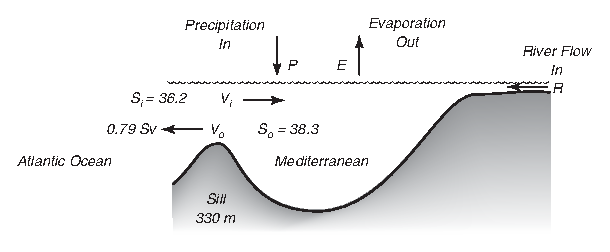
\includegraphics{basin}}
%% \centering
%% \footnotesize
%% Figure 7.1 Schematic \rule{0mm}{3ex}diagram of flow into and out 
%% of a basin.\\Values from Bryden and Kinder (1991).
%% 
%% \label{fig:basin}
%% \vspace{-1ex}
%% \end{figure}

Масса втекающей воды по определению равна, $\rho_i*V_i$. Согласно закону
сохранения массы:
\begin{equation}
\rho_i V_i = \rho_o V_o
\end{equation}
где, $\rho_i$, $\rho_o$~--- плотность втекающей и вытекающей
воды. Обычно мы можем принять их равными друг другу~$\rho_i = \rho_o$.  Если
выпадение осадков~$P$ и испарение~$E$ на поверхности бассейна, а $R$~---
привнос воды реками, то по закону сохранения массы:
\begin{equation}
V_i + R + P = V_o + E
\end{equation}
Разрешая для $(V_o - V_i)$:
\begin{equation}
V_o - V_i = (R + P) - E
\end{equation}

Согласно которой в среднем за достаточно большой промежуток времени
разница между втекающей и вытекающей водой должна находиться в балансе
с поступлением осадков плюс привнос воды реками минус испарение.
%
% The mass flowing out is, by definition, $\rho_o \, V_o$. If the volume
% of the sea does not change, conservation of mass requires:
% \begin{equation}
% \rho_i\,V_i = \rho_o\,V_o
% \end{equation}
% where, $\rho_i, \,\rho_o$ are the densities of the water flowing in and out.
% We can usually assume, with little error, that $\rho_i = \rho_o$.
%
% If there is precipitation $P$ and evaporation $E$ at the
% surface of the basin and river inflow $R$, conservation of mass becomes:
% \begin{equation}
% V_i + R + P = V_o + E
% \end{equation}
% Solving for ($V_o$ - $V_i$):
% \begin{equation}
% V_o - V_i = (R + P) - E
% \end{equation}
% which states that the net flow of water into the basin must balance
% precipitation plus river inflow minus evaporation when averaged over a
% sufficiently long time.

Так как соль в океане не осаждается и никаким другим способом из него
не пропадает уравнение сохранения соли будет иметь вид:
\begin{equation}
\rho_i V_i S_i = \rho_o V_o S_o
\end{equation}
Где $\rho_i$, $S_i$ плотность и солёность втекающей воды, а $rho_o$,
$S_o$ плотность и солёность ытекающей воды. Плотности мы снова можем
принять равными друг другу~$\rho_i = \rho_o$.
%
% Because salt is not deposited or removed from the sea, conservation of salt
% requires :
% \begin{equation}
% \rho_i\,V_i\,S_i = \rho_o\,V_o\,S_o
% \end{equation}
% Where $\rho_i$, $S_i$ are the density and salinity of the incoming water, 
% and $\rho_o$, $S_o$ are density and salinity of the outflow. With little
% error, we can again assume that $\rho_i$ = $\rho_o$.

%% Рисунок 7.1 Схематичное изображения потоков входящих и выходящих из
%% бассейна. Взято из Pickard and Emery, 1990

\begin{paragraph}{Пример применения закона сохранения масс и соли}
% \paragraph{An Example of Conservation of Mass and Salt}
Пиккард и Эмери (1990) в своей Описательной Физической океаногрфии
(Descriptive Physical oceanography) применили эту теорию к потоку в
Средиземном Море, используя значения солёности представленные на
рисунке 7.2. Входящий объём воды был оценён в 1.75*106 м3/с=1.75Св,
где Св=Свердруп=106 м3/с~--- единица объёма используемая в
океанографии. Решая уравнение 7.4 при условии что~$\rho_i = \rho_o$ и
используя оценённое значение~$V_i$ с измеренными значениями солёности
получим $Vo = 1.68 \times 10^6$~м3/с. Подставляя это значение в
формулу 7.3 получим~$(R + P -E) = -7 \times 10^4$~м3/с.
%
% Using the values for the flow at the Strait of Gibraltar measured by Bryden
% and Kinder (1991) and shown in figure 7.1, solving (7.4) for $V_i$ assuming
% that $\rho_i = \rho_o$, and using the estimated value of $V_o$, 
% gives $V_i = 0.836$ Sv $= 0.836 \times 10^6$ m$^3$/s, 
% where Sv = Sverdrup\index{Sverdrup} $= 10^6$ m$^3$/s is the unit of volume
% transport \index{transport!volume}used in oceanography. Using $V_i$ 
% and $V_o$ in (7.3) gives  $(R + P - E) = - 4.6 \times 10^4$ m$^3$/s.

Зная~$V_i$ мы также можем посчитать минимальное время обновления всей
воды моря. $T_m$ равняется объёму всей воды моря поделённому на объём
входящей воды. Объём Средиземного моря приблизительно~$4\times 10^6$~км3.  
Переводя $1.75\times 10^6$~м3/с в км3/год мы получим 
$-5.5 \times 10^4$~км3/год. Тогда 
$T_m = 4 \times 10^6\text{~км3}/-5.5 \times 10^4 \text{км3/год} = 70\text{ лет}$. 
Реальное время зависит от перемешивания в толще моря. Если воды хорошо
перемешаны, время полного обновления близко к минимальному, если нет
то оно больше.
%
% Knowing $V_i$ we can also calculate a minimum flushing time for replacing
% water in the sea by incoming water. The minimum flushing time $T_m$ is
% the volume of the sea divided by the volume of incoming water.
% The Mediterranean has a volume of around $4 \times 10^6$ km$^3$.
% Converting $0.836 \times 10^6$ m$^3$/s to km$^3$/yr we obtain
% $2.64 \times10^4$ km$^3$/yr. Then, 
% $T_m = 4 \times 10^6$ km$^3$/$2.64 \times 10^4$  km$^3$/yr $= 151$ yr. 
% The actual time depends on mixing\index{mixing!and flushing time} within
% the sea. If the waters are well mixed, the flushing time is close
% to the minimum time, if they are not well mixed, the flushing time is longer.

Наш пример с потоком в Средиземном море это вариант бокс модели (box
model). В этих моделях большие системы, такие как Средиземное море,
заменяют боксами. Жидкость, химические вещества или живые организмы
могут перемещаться между боксами, и уравнения сохранения используются
для того чтобы вызывать и контролировать различные взаимодействия
внутри системы.
%
% Our example of flow into and out of the Mediterranean Sea is an example
% of a \textit{box model}\index{box model|textbf}. A box model replaces
% large systems, such as the Mediterranean Sea, with boxes. Fluids or chemicals
% or organisms can move between boxes, and conservation equations are
% used to constrain the interactions within systems.
\end{paragraph}
\end{section}

%% \begin{figure}[b!]
%% %\vspace{-3ex}
%% 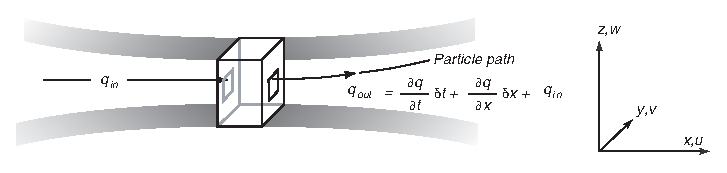
\includegraphics{derivativesketch}
%% \centering
%% \footnotesize
%% Figure 7.2 Sketch of flow \rule{0mm}{4ex}used for deriving the
%% total derivative.
%% 
%% \label{fig:derivativesketch}
%% \vspace{-3ex}
%% \end{figure}

\begin{section}{Полная производная}
% \section{The Total Derivative (D/Dt)}
Если число боксов в системе будет увеличивается до такого количества
что размер каждого бокса станет очень малым, мы в конце концов
достигнем предела используемого в дефференциальном
исчеслении. Например если мы разделим поток воды на боксы с ребром в
несколько метров, то сможем прийти к дефференциальным уравнениям
описывающим поток жидкости.
%
% \index{total derivative|textbf}If the number of boxes in a system increases
% to a very large number as the size of each box shrinks, we eventually
% approach limits used in differential calculus. For example, if we subdivide
% the flow of water into boxes a few meters on a side, and if we use
% conservation of mass, momentum, or other properties within each box,
% we can derive the differential equations governing fluid flow.

Рассмотрим простой пример ускорения движения потока в маленьком кубе
жидкости. Результирующее уравнение называется полной производной. Оно
связывает ускорение частицы воды с производной поля скорости в
фиксированной точке жидкости. Чтобы вывести уравнения движения
жидкости мы будем использовать Второй Закон Ньютона, который позволяет
расчитывать ускорение частиц проходящих через фиксированную точку в
жидкости.
%
% Consider the example of acceleration of flow in a small box of fluid. The
% resulting equation is called the \textit{total derivative}. It relates the
% acceleration of a particle $Du/Dt$ to derivatives of the velocity field at a
% fixed point in the fluid. We will use the equation to derive the equations 
% for fluid motion from Newton's Second Law which  requires calculating the
% acceleration of a particles passing a fixed point in the fluid.

%% Рисунок 7.3 Изображение потока использованное для вывода полной
%% производной.

Мы начнём с рассмотрения потока имеющего параметры qin на входе и qout
на выходе небольшого бокса, изображённого на рисунке 7.3.
Если $q$ может изменятся непрерывно в пространстве и времени, то
отношения между $q_{in}$ and $q_{out}$ будут иметь вид:
\begin{equation}
q_{out} = q_{in} + \frac{\partial{q}}{\partial{t}}\,\delta{t} + \frac{\partial{q}}{\partial{x}}\,\delta{x}
\end{equation}
Величина изменений параметра~$q$ внутри объёма будет равняться:
\begin{equation}
\frac{Dq}{Dt} = \frac{q_{out} - q_{in}}{\delta{t}}=
\frac{\partial{q}}{\partial{t}} +
\frac{\partial{q}}{\partial{x}}\frac{\delta{x}}{\delta{t}}
\end{equation}
Но $\delta x /\delta t$~--- это скорость~$u$; поэтому:
\begin{displaymath}
\frac{Dq}{Dt} = \frac{\partial{q}}{\partial{t}} +
u\frac{\partial{q}}{\partial{x}}
\end{displaymath}
В трёх измерениях полная производная принимает вид:
\begin{subequations}
\begin{align}
\frac{D}{Dt} = & \:\frac{\partial}{dt} + u\frac{\partial}{\partial{x}} + v\frac{\partial}{\partial y} + w\frac{\partial
}{\partial z}
\\
\frac{D}{Dt} = & \:\frac{\partial}{dt} +
\mathbf{u}\cdot \nabla(\,)
\end{align}
\end{subequations}
где $u$~--- вектор скорость а $\nabla$~--- опрератор дельта из теории
векторного поля. (См. Feynman, Leighton, and Sands 1964?: 2--6).
%
% We begin by considering the flow of a quantity  $q_{in}$ into and $q_{out}$
% out of the small box sketched in figure 7.2. If $q$ can change continuously
% in time and space, the relationship between $q_{in}$ and $q_{out}$ is:
% \begin{equation}
% q_{out} = q_{in} + \frac{\partial{q}}{\partial{t}}\,\delta{t} + \frac{\partial{q}}{\partial{x}}\,\delta{x}
% \end{equation}
% The rate of change of the quantity $q$ within the volume is:
% \begin{equation}
% \frac{Dq}{Dt} = \frac{q_{out} - q_{in}}{\delta{t}}=
% \frac{\partial{q}}{\partial{t}} +
% \frac{\partial{q}}{\partial{x}}\frac{\delta{x}}{\delta{t}}
% \end{equation}
% But $\delta x /\delta t$ is the velocity $u$, and therefore:
% \begin{displaymath}
% \frac{Dq}{Dt} = \frac{\partial{q}}{\partial{t}} +
% u\frac{\partial{q}}{\partial{x}}
% \end{displaymath}
% In three dimensions, the total derivative becomes:
% \begin{subequations}
% \begin{align}
% \frac{D}{Dt} = & \:\frac{\partial}{dt} + u\frac{\partial}{\partial{x}} + v\frac{\partial}{\partial y} + w\frac{\partial
% }{\partial z}
% \\
% \frac{D}{Dt} = & \:\frac{\partial}{dt} +
% \mathbf{u}\cdot \nabla(\,)
% \end{align}
% \end{subequations}
% where $\mathbf{u}$ is the vector velocity and $\nabla$ is the
% operator \textit{del} of vector field theory (See Feynman, Leighton, and Sands
% 1964: 2--6).

Это удивительный результат. Простое изменение системы координат
связанной с движущейся частицей на систему зафиксированную в
пространстве изменяет простую линейную производную на нелинейную
частную производную. Давайте теперь используем это уравнение чтобы
сосчитать изменение количества движения частицы жидкости.
%
% This is an amazing result. Transforming coordinates from one following
% a particle to one fixed in space converts a simple linear derivative
% into a non-linear partial derivative. Now let's use the equation to 
% calculate the change of momentum of a parcel of fluid.
\end{section}

\begin{section}{Уравнение количества движения}
% \section{Momentum Equation}
Второй Закон Ньютона связывает изменение количества движения жидкости
с приложенной к ней силой. Изменения имеют вид:
\begin{equation}
\frac{D(m\textbf{v})}{Dt} = \textbf{F}
\end{equation}
Где \textbf{F}~--- сила, \textbf{v}~--- скорость а~$m$~---
масса. Здесь мы должны использовать полную производную, так как мы
расчитываем силу для частицы жидкости. Мы можем принять массу
постоянной и написать:
\begin{equation}
\frac{D\textbf{v}}{Dt} = \frac{\textbf{F}}{m} = \textbf{f$_m$}
\end{equation}
где f$_m$~--- это сила действующая на единицу массы (массовая сила)
%
% \index{momentum equation}Newton's Second Law relates the change of
% the momentum of a fluid mass due to an applied force. The change
% is:
% \begin{equation}
% \frac{D(m\textbf{v})}{Dt} = \textbf{F}
% \end{equation}
% where \textbf{F} is force, $m$ is mass, and \textbf{v} is velocity. 
% I have emphasized the need to use the total derivative because we are 
% calculating the force on a particle. We can assume that the mass is constant,
% and (7.8) can be written:
% \begin{equation}
% \frac{D\textbf{v}}{Dt} = \frac{\textbf{F}}{m} = \textbf{f$_m$}
% \end{equation}
% where \textbf{f$_m$} is force per unit mass.

Для нас важны четыре силы: градиента давления, Cила Кориолиса, Cила
Тяжести и Сила Трения. Не раскрывая вид этих сил (их производные будут
рассмотрены в следующем блоке) можно записать что:
\begin{equation}
\frac{D\mathbf{v}}{Dt} = -\,\frac{1}{\rho}\nabla\,p -
\,2\boldsymbol{\Omega}
\times \mathbf{v} + \mathbf{g} + \mathbf{F_r}
\end{equation}
Ускорение равно отрицательному градиенту давления минус сила Кориолиса
плюс сила тяжести плюс другие силы. Здесь $g$~--- ускорение силы
тяжести, $F_r$~--- сила трения, а $\boldsymbol{\Omega}$~--- угловая
скорость вращения Земли ($2\pi$ разделить на 24 часа)
\begin{equation}
\boxed{\Omega = 7.292 \times 10^{-5} \text{ radians/s}}
\end{equation}
%
% Four forces are important: pressure gradients, Coriolis force, gravity, and
% friction. Without deriving the form of these forces (the derivations are 
% given in the next section), we can write (7.9) in the following form.
% \begin{equation}
% \frac{D\mathbf{v}}{Dt} = -\,\frac{1}{\rho}\nabla\,p -
% \,2\boldsymbol{\Omega}
% \times \mathbf{v} + \mathbf{g} + \mathbf{F_r}
% \end{equation}
% Acceleration equals the negative pressure gradient minus the Coriolis force 
% plus gravity plus other forces. Here \textbf{g} is acceleration of gravity, 
% $\mathbf{F_r}$ is friction, and the magnitude $\Omega$ 
% of $\boldsymbol{\Omega}$ is the \textit{Rotation Rate of earth}\index{earth!rotation
% rate|textbf}, 2$\pi$ radians per sidereal day or
% \begin{equation}
% \fbox{$\D
% \Omega = 7.292 \times 10^{-5} \text{ radians/s} $}
% \end{equation}

\begin{paragraph}{Уравнение количества движения в прямоугольной системе координат:}
% \paragraph{Momentum Equation in Cartesian coordinates:}
Раскрыв производные и переписав компоненты уравнения (7.10) в
прямоугольной системе координат получим Уравнение движения.
\begin{subequations}
\begin{align}
\frac{\partial{u}}{\partial{t}} + u\,\frac{\partial{u}}{\partial{x}}
+ v\,\frac{\partial{u}}{\partial{y}} +w\,\frac{\partial{u}}{\partial{z}} &=
-\,\frac{1}{\rho}\,\frac{\partial{p}}{\partial{x}} +
2\,\Omega\,{v}\,\sin\varphi +  F_x \\
 \frac{\partial{v}}{\partial{t}} + u\,\frac{\partial{v}}{\partial{x}} +
v\,\frac{\partial{v}}{\partial{y}} +w\,\frac{\partial{v}}{\partial{z}} &=
-\,\frac{1}{\rho}\,\frac{\partial{p}}{\partial{y}} - 2\,\Omega\,u\,\sin\varphi
+ F_y
\\
 \frac{\partial{w}}{\partial{t}} + u\,\frac{\partial{w}}{\partial{x}} +
v\,\frac{\partial{w}}{\partial{y}} +w\,\frac{\partial{w}}{\partial{z}} &=
-\,\frac{1}{\rho}\,\frac{\partial{p}}{\partial{z}} + 2\,\Omega\,{u}\,\cos\varphi
- g + F_z
\end{align}
\end{subequations}
Где~$F_i$~--- компоненты всех сил трения действующих на единицу массы
и $\varphi$~--- широта. К тому же мы предполагаем что $w<<v$, поэтому
член $2\,\Omega\,w \cos \varphi$ исключён их уравнения 7.12а.
%
% \index{momentum equation!Cartesian coordinates|textbf}Expanding the 
% derivative in (7.10) and writing the components in a Cartesian coordinate 
% system gives the \textit{Momentum Equation}:
% \begin{subequations}
% \begin{align}
% \frac{\partial{u}}{\partial{t}} + u\,\frac{\partial{u}}{\partial{x}}
% + v\,\frac{\partial{u}}{\partial{y}} +w\,\frac{\partial{u}}{\partial{z}} &=
% -\,\frac{1}{\rho}\,\frac{\partial{p}}{\partial{x}} +
% 2\,\Omega\,{v}\,\sin\varphi +  F_x \\
%  \frac{\partial{v}}{\partial{t}} + u\,\frac{\partial{v}}{\partial{x}} +
% v\,\frac{\partial{v}}{\partial{y}} +w\,\frac{\partial{v}}{\partial{z}} &=
% -\,\frac{1}{\rho}\,\frac{\partial{p}}{\partial{y}} - 2\,\Omega\,u\,\sin\varphi
% + F_y
% \\
%  \frac{\partial{w}}{\partial{t}} + u\,\frac{\partial{w}}{\partial{x}} +
% v\,\frac{\partial{w}}{\partial{y}} +w\,\frac{\partial{w}}{\partial{z}} &=
% -\,\frac{1}{\rho}\,\frac{\partial{p}}{\partial{z}} + 2\,\Omega\,{u}\,\cos\varphi
% - g + F_z
% \end{align}
% \end{subequations}
% where $F_i$ are the components of any frictional force per unit mass, and
% $\varphi$ is latitude. In addition, we have assumed that $w << v$, so the
% $2\,\Omega\,w \cos \varphi$ has been dropped from equation in (7.12a).

Уравнение 7.12 называют по разному. Леонард Эйлер (1707--1783) первым
записал его в общем виде для потока жидкости с внутренними силами,
поэтому иногда оно называется уравнением Эйлера или уравнением
ускорения. Луис Мария Генри Навье (1785--1836) добавил силы трения и
теперь уравнение иногда называют Уравнение Навье Стокса.
%
% Equation (7.12) appears under various names. Leonhard Euler (1707--1783)
% first wrote out the general form for fluid flow with external forces,
% and the equation is sometimes called the
% \textit{Euler equation}\index{Euler equation} or the
% \textit{acceleration equation}\index{acceleration equation}. Louis Marie
% Henri Navier (1785--1836) added the frictional terms, and so the equation
% is sometimes called the \textit{Navier-Stokes equation}\index{Navier-Stokes
% equation}.

Член $2\,\Omega\,u\, \cos{\varphi}$ в уравнении 7.12 с гораздо
меньше~$g$, поэтому им можно пренебрегать при описании динамики
океана. Но этого не следует делать при измерениях силы тяжести
гравиметрами с движущихся кораблей.
%
% The term $2\,\Omega\,u\, \cos{\varphi}$ in (7.12c) is small compared with $g$,
% and it can be ignored in ocean dynamics. It cannot be ignored, however, for
% gravity surveys made with gravimeters on moving ships.
%
\end{paragraph}

%% \begin{figure}[h!]
%% \makebox[121mm][c]{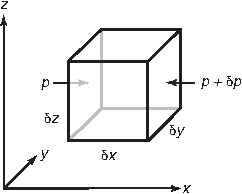
\includegraphics{pressuresketch}}
%% \centering
%% \footnotesize
%% Figure 7.3 Sketch of flow \rule{0mm}{3ex}used for deriving the
%% pressure term in the momentum equation.
%% 
%% \label{fig:pressuresketch}
%% \vspace{-3ex}
%% \end{figure}
%% Рисунок 7.4 Изображение потока использованное для вывода члена
%% плотности в уравнении количества движения.

\begin{paragraph}{Производная члена (элемента) давления.}
% \paragraph{Derivation of Pressure Term}
Рассмотрим силы действующие на стороны маленького кубика
жидкости. Равнодействующая сила~$\delta F_x$ в направлении~$x$ равна:
\begin{align}
\delta F_x &= p\,\delta{y}\,\delta{z} - (p + \delta{p})\,\delta{y}\,\delta{z}
\notag \\
\delta F_x &= - \delta{p}\,\delta{y}\,\delta{z} \notag
\end{align}
но
\begin{displaymath}
\delta{p} = \frac{\partial{p}}{\partial{x}}\,\delta{x}
\end{displaymath}
и поэтому
\begin{align}
\delta F_x &= - \frac{\partial{p}}{\partial{x}}\,\delta{x}\,\delta{y}\,\delta{z}
\notag \\
\delta F_x &=-\,\frac{\partial{p}}{\partial{x}}\, \delta{V} \notag
\end{align}
При делении на массу воды находящуюся в боксе $\delta m$, ускорение
жидкости по оси~$x$ составит:
\begin{equation}
a_x = \frac{{\delta F_x}}{\delta{m}} = - \frac{\partial{p}}{\partial{x}}\,
\frac{\delta{V}}{\delta{m}} \notag
\end{equation}
\begin{equation}
\boxed{a_x = - \frac{1}{\rho}\,\frac{\partial{p}}{\partial{x}}}
\end{equation}
Силы давления и ускорения этими силами вызываемые по осям~$y$ и~$z$
выводятся подобным образом.
%
% Consider the forces acting on the sides of a small cube of fluid (figure 7.3).
% The net force $\delta F_x$ in the $x$ direction is
% \begin{align}
% \delta F_x &= p\,\delta{y}\,\delta{z} - (p + \delta{p})\,\delta{y}\,\delta{z}
% \notag \\
% \delta F_x &= - \delta{p}\,\delta{y}\,\delta{z} \notag
% \end{align}
% But
% \begin{displaymath}
% \delta{p} = \frac{\partial{p}}{\partial{x}}\,\delta{x}
% \end{displaymath}
% and therefore
% \begin{align}
% \delta F_x &= - \frac{\partial{p}}{\partial{x}}\,\delta{x}\,\delta{y}\,\delta{z}
% \notag \\
% \delta F_x &=-\,\frac{\partial{p}}{\partial{x}}\, \delta{V} \notag
% \end{align}
% Dividing by the mass of the fluid $\delta m$ in the box, the acceleration of
% the fluid in the $x$ direction is:
% \begin{equation}
% a_x = \frac{{\delta F_x}}{\delta{m}} = - \frac{\partial{p}}{\partial{x}}\,
% \frac{\delta{V}}{\delta{m}} \notag
% \end{equation}
% \begin{equation}
% \boxed{a_x = - \frac{1}{\rho}\,\frac{\partial{p}}{\partial{x}}}
% \end{equation}
% The pressure forces and the acceleration due to the pressure forces in 
% the $y$ and $z$ directions are derived in the same way.
\end{paragraph}

\begin{paragraph}{Сила Kориолиса в уравнении движения}
% \paragraph{The Coriolis Term in the Momentum Equation}
Член силы кориолиса присутствует потому что мы описываем течения на
вращающейся Земле. Производная Силы кориолиса очень сложна. Генри
Стоммел (Henry Stommel), знаменитый океанограф из Океанографического
Института в Вудс Холе (Woods Hole Oceanographic Institution) вместе с
Денисом Муром (Dennis Moore) посвятили ей целую книгу (Stommel \& Moore, 1989).
%
% \index{Coriolis force}\index{momentum equation!Coriolis term}The Coriolis
% term exists because we describe currents in a reference frame fixed on earth.
% The derivation of the Coriolis terms is not easy. Henry Stommel, the noted
% oceanographer at the Woods Hole Oceanographic Institution even wrote a book
% on the subject with Dennis Moore (Stommel \& Moore, 1989).

Обычно мы утверждаем что массовая сила, ускорение частицы жидкости, во
вращающейся системе координат будет записано как:
\begin{equation}
\textbf{a}_{fixed} = \left(\frac{D\textbf{v}}{Dt}\right)_{fixed} =
 \left(\frac{D\textbf{v}}{Dt}\right)_{rotating} + \left( 2 \boldsymbol{\Omega}
\times \mathbf{v} \right) + \boldsymbol{\Omega} \times \left(
\boldsymbol{\Omega} \times \mathbf{R} \right)
\end{equation}
Где $R$~--- векторное расстояние от центра
Земли. $\boldsymbol{\Omega}$~--- угловой вектор скорости Земли а
$v$~--- скорость частицы жидкости в координатах зафиксированных на
земле. Член $2 \boldsymbol{\Omega} \times \mathbf{v}$~--- сила
Кориолиса, а $\boldsymbol{\Omega} \times \left( \boldsymbol{\Omega}
\times \mathbf{R} \right)$~--- центробежное ускорение. Последний член
включён в силу тяжести (рис 7.5).
%
% Usually, we just state that the force per unit mass, the acceleration 
% of a parcel of fluid in a rotating system, can be written:
% \begin{equation}
% \textbf{a}_{fixed} = \left(\frac{D\textbf{v}}{Dt}\right)_{fixed} =
%  \left(\frac{D\textbf{v}}{Dt}\right)_{rotating} + \left( 2 \boldsymbol{\Omega}
% \times \mathbf{v} \right) + \boldsymbol{\Omega} \times \left(
% \boldsymbol{\Omega} \times \mathbf{R} \right)
% \end{equation}
% where \textbf{R} is the vector distance from the center of earth,
% $\boldsymbol{\Omega}$ is the angular velocity vector of earth,
% and \textbf{v} is the velocity of the fluid parcel in coordinates fixed to earth.
% The term $2 \boldsymbol{\Omega} \times \mathbf{v}$ is the Coriolis force, and the
% term $\boldsymbol{\Omega} \times \left( \boldsymbol{\Omega} \times \mathbf{R}
% \right)$ is the centrifugal acceleration. The latter term is included in gravity
% (figure 7.4).
\end{paragraph}

\begin{paragraph}{Сила Тяжести в уравнении движения}
% \paragraph{The Gravity Term in the Momentum Equation}
Гравитационное притяжение между двумя массами~$M_1$ и~$m$, выражается
формулой:
\begin{displaymath}
\textbf{F}_g = \frac{G\,M_1\, m}{R^2}
\end{displaymath}
Где $R$~--- расстояние между массами, а $G$~--- гравитационная
постоянная. Вектор силы тяжести~$F_g$ действует вдоль линии
соединяющей центры масс. 
%
% \index{momentum equation!gravity term}The gravitational attraction
% of two masses $M_1$ and $m$ is:
% \begin{displaymath}
% \textbf{F}_g = \frac{G\,M_1\, m}{R^2}
% \end{displaymath}
% where $R$ is the distance between the masses, and $G$ is the gravitational
% constant. The vector force $\textbf{F}_g$ is along the line connecting the two
% masses.

Сила тяжести действующая на единицу массы будет равна:
\begin{equation}
\frac{\textbf{F}_g}{m} = \textbf{g}_f =\frac{G\,M_E}{R^2}
\end{equation}
Где $M_E$~--- масса Земли. Добавив центробежное ускорение в (7.15)
получим тяготение~$g$ (рис 7.5)
\begin{equation}
\textbf{g} = \textbf{g}_f - \boldsymbol{\Omega} \times
\left( \boldsymbol{\Omega} \times \mathbf{R}
\right)
\end{equation}
%
% The force per unit mass due to gravity is:
% \begin{equation}
% \frac{\textbf{F}_g}{m} = \textbf{g}_f =\frac{G\,M_E}{R^2}
% \end{equation}
% where $M_E$ is the mass of earth. Adding the centrifugal acceleration 
% to (7.15) gives gravity $\textbf{g}$ (figure 7.4):
% \begin{equation}
% \textbf{g} = \textbf{g}_f - \boldsymbol{\Omega} \times
% \left( \boldsymbol{\Omega} \times \mathbf{R}
% \right)
% \end{equation}

Отметим что сила тяжести не направлена к центру масс
Земли. Центробежное ускорение заставляет грузик отвеса отклонятся под
небольшим углом от линии проходящей через Земной центр масс. В
результате форма Земли представляет собой не сферу а сплюснутый с двух
сторон элипсоид. Земля это вращающаяся жидкая планета имеющая
выпуклость в районе экватора.
%
% Note that gravity does not point toward earth's center of mass. The 
% centrifugal acceleration causes a plumb bob to point at a small angle
% to the line directed to earth's center of mass. As a result, earth's surface
% including the ocean's surface is not spherical but it is a oblate ellipsoid.
% A rotating fluid planet has an equatorial bulge.
\end{paragraph}

%% \begin{figure}[h!]
%% \makebox[120mm][c]{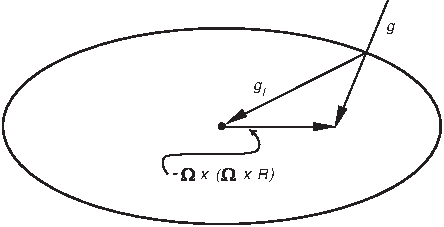
\includegraphics{gravitysketch}}
%% \footnotesize
%% Figure 7.4 Downward \rule{0mm}{4ex}acceleration $g$ of a body at
%% rest on earth's surface is the sum of gravitational acceleration between the body
%% and earth's mass $g_f$ and the centrifugal acceleration due to earth's
%% rotation $\Omega\times(\Omega\times{R})$. The surface of an ocean at
%% rest must be perpendicular to $g$, and such a surface is close to an
%% ellipsoid of rotation. earth's ellipticity is greatly exaggerated here.
%% \label{fig:gravitysketch}
%% \vspace{-2ex}
%% \end{figure}

%% Рисунок 7.5 Ускорение g тела на поверхности Земли как сумма ускорения
%% свободного падения между телом и Землё~--- gf и центробежного
%% ускорения вызванного вращением Земли W x (Wx R). Невзволнованная
%% поверхность океана должна быть перпендикулярна g и имеет форму
%% элипсоида вращения. Элиптичность Земли здесь сильно преувеличена.
\end{section}

\begin{section}{Закон Сохранения Массы: уравнение неразрывности}
% \section{Conservation of Mass: The Continuity Equation}
Теперь давайте выведем уравнение сохранения массы для жидкости. Начнём
с того что опишем потоки массы идущие внутрь и наружу маленького
куба. (рис 7.6)
\begin{align}
\text{Mass flow in} &= \rho \, u \, \delta z \, \delta y \notag  \\
\text{Mass flow out} &= (\rho + \delta \rho ) (u + \delta u) \delta z \,  \delta y \notag
\end{align}

Рисунок 7.6 Изображение потока использованное для вывода уравнения
неразрывности

Изменение массы внутри объёма должно быть равно (поток массы
внутрь)-(поток массы наружу)
\begin{equation}
\text{Mass flux} = \left(\rho \, \frac{\partial{u}}{\partial{x}} + u\,\frac{\partial{\rho}}{\partial{x}}
+\frac{\partial{\rho}}{\partial{x}}\,\frac{\partial{u}}{\partial{x}}\,\delta{x}\right)\delta{x}\,\delta{y}\,\delta{z}
\notag
\end{equation}

Третий член в круглых скобках становится гораздо меньше чем первые
два, так как $\delta x \rightarrow 0$ и
\begin{equation}
\text{Mass flux} =
\frac{\partial{(\rho{u})}}{\partial{x}}\,\delta{x}\,\delta{y}\,\delta{z} \notag
\end{equation}
переписывая по осям (в трёх измерениях)
\begin{displaymath}
\mbox{Mass flux} = \left(\frac{\partial{(\rho{u})}}{\partial{x}} +
\frac{\partial{(\rho{v})}}{\partial{y}} +
\frac{\partial{(\rho{w})}}{\partial{z}}\right)\delta{x}\,\delta{y}\,\delta{z}
\end{displaymath}
Изменение массы внутри объёма будет равно:
\begin{displaymath}
\frac{\partial\rho}{\partial{t}}\,\delta{x}\,\delta{y}\,\delta{z}
\end{displaymath}
И по закону сохранения массы общее изменение массы должно быть равно нулю:
\begin{equation}
\frac{\partial\rho}{\partial{t}} + \frac{\partial{(\rho{u})}}{\partial{x}} + \frac{d(\rho{v})}{\partial{y}} + \frac{\partial{(\rho{w})}}{\partial{z}} = 0
\end{equation}

Это уравнение неразрывности для сжимаемой жидкости, впервые выведенное
Леонардом Эёлером (1707--1783).
%
% \index{conservation of mass}\index{continuity equation}Now let's
% derive the equation for the conservation of mass in a fluid. We
% begin by writing down the flow of mass into and out of a small box
% (figure 7.5).
%% \begin{figure}[h!]
%% \makebox[120mm][c]{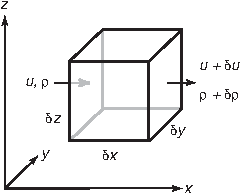
\includegraphics{continuitysketch}}
%% \centering
%% \footnotesize
%% Figure 7.5 Sketch of flow \rule{0mm}{4ex}used for deriving the
%% continuity equation.
%% \label{fig:continuitysketchR}
%% \vspace{-3ex}
%% \end{figure}
% \begin{align}
% \text{Mass flow in} &= \rho \, u \, \delta z \, \delta y \notag  \\
% \text{Mass flow out} &= (\rho + \delta \rho ) (u + \delta u) \delta z \,  \delta y \notag
% \end{align}
% The mass flux into the volume must be (mass flow out) $-$ (mass flow
% in). Therefore,
% \begin{equation}
% \text{Mass flux} = ( \rho \, \delta u + u \, \delta \rho + \delta \rho \, \delta u)  \delta z \,  \delta y \notag
% \end{equation}
% But
% \begin{equation}
% \delta u = \frac{\partial u}{\partial x} \delta x \,;\quad \delta \rho = \frac{\partial {\rho}}{\partial x} \delta x \notag
% \end{equation}
% Therefore
% \begin{equation}
% \text{Mass flux} = \left(\rho \, \frac{\partial{u}}{\partial{x}} + u\,\frac{\partial{\rho}}{\partial{x}}
% +\frac{\partial{\rho}}{\partial{x}}\,\frac{\partial{u}}{\partial{x}}\,\delta{x}\right)\delta{x}\,\delta{y}\,\delta{z}
% \notag
% \end{equation}
% The third term inside the parentheses becomes much smaller than the first two terms
% as $\delta x \rightarrow 0$, and
% \begin{equation}
% \text{Mass flux} =
% \frac{\partial{(\rho{u})}}{\partial{x}}\,\delta{x}\,\delta{y}\,\delta{z} \notag
% \end{equation}
% In three dimensions:
% \begin{displaymath}
% \mbox{Mass flux} = \left(\frac{\partial{(\rho{u})}}{\partial{x}} +
% \frac{\partial{(\rho{v})}}{\partial{y}} +
% \frac{\partial{(\rho{w})}}{\partial{z}}\right)\delta{x}\,\delta{y}\,\delta{z}
% \end{displaymath}
% The mass flux must be balanced by a change of mass inside the volume, which is:
% \begin{displaymath}
% \frac{\partial\rho}{\partial{t}}\,\delta{x}\,\delta{y}\,\delta{z}
% \end{displaymath}
% and conservation of mass requires:
% \begin{equation}
% \frac{\partial\rho}{\partial{t}} + \frac{\partial{(\rho{u})}}{\partial{x}} + \frac{d(\rho{v})}{\partial{y}} + \frac{\partial{(\rho{w})}}{\partial{z}} = 0
% \end{equation}
% This is the \textit{continuity equation}\index{continuity equation|textbf} for compressible flow, first derived by
% Leonhard Euler (1707--1783).

Раскрыв производные и переместив слагаемые мы можем переписать
уравнение в форме:
\begin{displaymath}
\frac{\partial{\rho}}{\partial{t}} + u\,\frac{\partial{\rho}}{\partial{x}} + v\,\frac{\partial{\rho}}{\partial{y}} + w\,\frac{\partial{\rho}}{\partial{z}} +
\rho\,\frac{\partial{u}}{\partial{x}} + \rho\,\frac{\partial{v}}{\partial{y}} + \rho\,\frac{\partial{w}}{\partial{z}} = 0
\end{displaymath}
Первые четыре члена~--- это полная производная $D\rho/Dt$ из уравнения
(7.7), следовательно мы можем переписать (7.17) как :
\begin{equation}
\boxed{\frac{1}{\rho}\frac{D\rho}{Dt} + \frac{\partial{u}}{\partial{x}} + \frac{\partial{v}}{\partial{y}} + \frac{\partial{w}}{\partial{z}} = 0}
\end{equation}
Это другая форма записи уравнения неразрывности для сжимаемой жидкости.
%
% The equation can be put in an alternate form by expanding the derivatives of
% products and rearranging terms to obtain:
% \begin{displaymath}
% \frac{\partial{\rho}}{\partial{t}} + u\,\frac{\partial{\rho}}{\partial{x}} + v\,\frac{\partial{\rho}}{\partial{y}} + w\,\frac{\partial{\rho}}{\partial{z}} +
% \rho\,\frac{\partial{u}}{\partial{x}} + \rho\,\frac{\partial{v}}{\partial{y}} + \rho\,\frac{\partial{w}}{\partial{z}} = 0
% \end{displaymath}
% The first four terms constitute the total derivative of density $D\rho/Dt$ 
% from (7.7), and we can write (7.17) as:
% \begin{equation}
% \fbox{$\D
% \frac{\D1}{\D\rho}\frac{\D{D}\D\rho}{\D{Dt}} + \frac{\D\partial{u}}{\D\partial{x}} + \frac{\D\partial{v}}{\D\partial{y}} + \frac{\D\partial{w}}{\D\partial{z}} =
% 0
% $}\end{equation}
% This is the alternate form for the continuity equation for a compressible 
% fluid.

\begin{paragraph}{Приближение Буссинеска}
% \paragraph{The Boussinesq Approximation}
Плотность очень мало изменяется в океанах, поэтому Джозеф Буссинеск
(1842--1929), не тем будь помянут, предположил что мы можем принять
её постоянной (кроме случаев когда мы расчитываем давление в океанах
умножая её на $g$). Это сильно упрощает уравнение движения. 
%
% \index{Boussinesq approximation}Density is nearly constant in the
% ocean, and Joseph Boussinesq (1842--1929) noted that we can safely
% assume density is constant except when it is multiplied by $g$ in
% calculations of pressure in the ocean. The assumption greatly
% simplifies the equations of motion.

Буссинеск ввёл следующие условия:
% Boussinesq's assumption requires that:
\begin{enumerate}
\item
Скорости в океане должны быть гораздо меньше скорости звука~$c$. Это
даёт гарантию того что скорость не изменяет плотность. Если скорость
достигает скорости звука, она может приводить к серьёзным изменениям
плотности, таким как ударные волны.
%
% \vitem Velocities in the ocean must be small compared to the speed of
% sound\index{sound!speed!and Boussinesq approximation}
% $c$. This ensures that velocity does not change the density. As velocity
% approaches the speed of sound, the velocity field can produces large 
% changes of density such as shock waves.

\item
Фазовая скорость волн должна быть гораздо меньше~$c$. Скорость звука в
несжимаемой жидкости бесконечно большая и при рассмотрении звука в
океане мы должны предполагать жидкость сжимаемой. Это приближение не
работает для звуковых волн, но у всех других волн в океане скорости
гораздо меньше.
%
% \vitem The phase speed of waves or disturbances must be small compared 
% with $c$. Sound speed\index{sound!speed!in incompressible fluid} in
% incompressible flows is infinite, and we must assume the fluid is
% compressible when discussing sound in the ocean. Thus the approximation
% is not true for sound. All other waves in the ocean have speeds small
% compared to sound.

\item
Вертикальный масштаб движения должен быть гораздо меньше чем~$c^2/g$,
где~$g$~--- сила тяжести. Это обеспечивает то что давление с глубиной
увеличивается, а увеличение давления вызывает очень небольшие
изменения плотности.
%
% \vitem The vertical scale of the motion must be small compared
% with $c^2$/$g$, where $g$ is gravity. This ensures that as pressure increases
% with depth in the ocean, the increase in pressure produces only small changes
% in density.
\end{enumerate}

Эти условия выполняются для всех океанских потоков и обеспечивают
возможность рассмотрения воды как несжимаемой. Смотрите также Kundu
(1990: 79 and 112), Gill (1982: 85),Batchelor (1967: 167), или другие
тексты по гидромеханике, где более полно описано это приближение.
%
% The approximations are true for oceanic flows, and they ensure that oceanic
% flows are incompressible. See Kundu (1990: 79 and 112), Gill (1982: 85),
% Batchelor (1967: 167), or other texts on fluid dynamics for a more complete
% description of the approximation.
\end{paragraph}

\begin{paragraph}{Сжимаемость.}
% \paragraph{Compressibility}
Приближение Буссинеска предполагает что морская вода
несжимаема. Теперь давайте посмотрим каким образом это упрощает
уравнение неразрывности. Мы введём Коэффициент Сжимаемости:
\begin{displaymath}
\beta \equiv -\frac{1}{V}\,\frac{\partial{V}}{\partial{p}} =
-\frac{1}{V}\,\frac{dV}{dt}\Big/\frac{dp}{dt}
\end{displaymath}
где $V$~--- объём и $p$~--- давление. Для несжимаемой жидкости
$\beta = 0$, и :
\begin{displaymath}
\frac{1}{V}\,\frac{dV}{dt} = 0
\end{displaymath}
так как $dp$/$dt$ не равно 0. Вспоминая что плотность это масса
поделённая на единицу объёма, а масса постоянна, запишем:
\begin{displaymath}
\frac{1}{V}\frac{dV}{dt} = -\,V\frac{d}{dt}\left(\frac{1}{V}\right) =
- \frac{V}{m}\,\frac{d}{dt}\left(\frac{m}{V}\right)
=\,-\,\frac{1}{\rho}\,\frac{d\rho}{dt} =\,-\,\frac{1}{\rho}\, \frac{D\rho}{Dt} = 0
\end{displaymath}
следовательно (7.18) принимает вид:
\begin{equation}
\boxed{
 \frac{\partial{u}}{\partial{x}} + \frac{\partial{v}}{\partial{y}} + \frac{\partial{w}}{\partial{z}} = 0
}
\end{equation}
Это Уравнение Неразрывности для несжимаемой жидкости.
%
% \index{water!compressibility coefficient|textbf}The Boussinesq approximation
% is equivalent to assuming sea water is incompressible. Now let's see how the
% assumption simplifies the continuity equation. We define the
% \textit{coefficient of compressibility}
% \begin{displaymath}
% \beta \equiv -\frac{1}{V}\,\frac{\partial{V}}{\partial{p}} =
% -\frac{1}{V}\,\frac{dV}{dt}\Big/\frac{dp}{dt}
% \end{displaymath}
% where $V$ is volume, and $p$ is pressure. For incompressible flows, 
% $\beta$ = 0,
% and:
% \begin{displaymath}
% \frac{1}{V}\,\frac{dV}{dt} = 0
% \end{displaymath}
% because $dp$/$dt$ $\not=$ 0. Remembering that density is mass
% $m$ per unit volume $V$, and that mass is constant:
% \begin{displaymath}
% \frac{1}{V}\frac{dV}{dt} = -\,V\frac{d}{dt}\left(\frac{1}{V}\right) =
% - \frac{V}{m}\,\frac{d}{dt}\left(\frac{m}{V}\right)
% =\,-\,\frac{1}{\rho}\,\frac{d\rho}{dt} =\,-\,\frac{1}{\rho}\, \frac{D\rho}{Dt} = 0
% \end{displaymath}
% If the flow is incompressible, (7.18) becomes:
% \begin{equation}
% \fbox{$ \D
% \frac{\D\partial{u}}{\D\partial{x}} + \frac{\D\partial{v}}{\D\partial{y}} + \frac{\D\partial{w}}{\D\partial{z}} = 0 $}
% \end{equation}
% This is the \index{continuity equation} \textit{Continuity Equation for
% Incompressible Flows}.
\end{paragraph}
\end{section}

\begin{section}{Решения для уравнения движения}
% \section{Solutions to the Equations of Motion}
У нас есть четыре уравнения~--- три компонента из уровнения сохранения
количества движения и плюс уравнение неразрывности с четырьмя
неизвесными $u$, $v$, $w$, $p$. В принципе мы должны суметь решить эту
систему с заданными граничными условиями.  Но следует учесть что это
нелинейные частно-дефференциальные уравнения. Закон сохранения
количества движения применённый к жидкости превращает уравнение для
скорости из простого монотонного дифференциальное урвнения первого
порядка, которое обычно просто решается, в нелинейное уравнение в
частных производных, которое практически невозможно решить.
%
% Equations (7.12) and (7.19) are four equations, the three components of
% the momentum equation plus the continuity equation, with four unknowns: 
% $u$, $v$, $w$, $p$. Note, however, that these are non-linear partial
% differential equations. Conservation of momentum, when applied to a fluid,
% converted a simple, first-order, ordinary, differential equation for
% velocity (Newton's Second Law), which is usually easy to solve, into a
% non-linear partial differential equation, which is almost impossible to solve.

\begin{paragraph}{Граничные условия;}
% \paragraph{Boundary Conditions:}
В гидромеханике мы обычно принимаем что :
% In fluid mechanics, we generally assume:
\begin{enumerate}
\item
Нет скорости нормальной к границе, что значит отсутствие течения через
границу.
%
% \vitem No velocity normal to a boundary, which means there is no flow 
% through the boundary; and

\item
Нет течения праллельного твёрдой (сплошной) границе, что значит
отсутствие скольжения на твёрдой границе.
%
% \vitem No flow parallel to a solid boundary, which means no slip at the
% solid boundary.
\end{enumerate}
\end{paragraph}

\begin{paragraph}{Решения}
% \paragraph{Solutions}
Мы ожидаем что система их четырёх уравнений с четырьмя неизвестными
будет разрешима в принципе. Но на практике трудно найти решения даже
для простейших потоков. Во первых, насколько мне известно, не
существует точных решений для уравнений с трением. Существует только
несколько точных решений для уравнений без трения. Те кто интересуется
волнами в океане могут знать что одним из таких решений является
решение Герстнера (Gerstner) для волн на воде (Lamb, 1945: 251). Чтобы
решить эти уравнения мы должны их кардинальным образом упростить. Даже
численные расчёты для них сложны.
%
% We expect that four equations in four unknowns plus boundary conditions
% give a system of equations that can be solved in principle. In practice,
% solutions are difficult to find even for the simplest flows. First, as far
% as I know, there are no exact solutions for the equations with friction.
% There are very few exact solutions for the equations without friction.
% Those who are interested in ocean waves might note that one such exact
% solution is Gerstner's solution for water waves (Lamb, 1945: 251). Because
% the equations are almost impossible to solve, we will look for ways to
% greatly simplify the equations. Later, we will find
% that even numerical calculations are difficult.

Аналитические решения могут быть найдены для большинства упрощённых
форм уравнения движения. Такие решения используются для изучения
различных процессов в океане, включая волны. Решения для потоков в
океане с реальным побережьем и элементами дна должны находится при
помощи численных методов. В следующих главах мы будем использовать
решения для упрощённых форм уравнений. В главе 16 мы обсудим численные
решения.
%
% Analytical solutions can be obtained for much simplified forms of the 
% equations of motion. Such solutions are used to study processes in the ocean,
% including waves. Solutions for oceanic flows with realistic coasts and
% bathymetric features must be obtained from numerical solutions. In the next
% few chapters we seek solutions to simplified forms of the equations.
% In Chapter 15 we will consider numerical solutions.
\end{paragraph}
\end{section}

\begin{section}{Основные концепции}
% \section{Important Concepts}
\begin{enumerate}
\item
Сила тяжести, сила плавучести и сила ветра~--- главные силы
действующие в океане.
%
% \item Gravity, buoyancy\index{buoyancy}, and wind are the dominant forces 
% acting on the ocean.

\item
Вращение земли вызывает псевдо силу~--- силу Кориолиса.
%
% \vitem Earth's rotation produces a pseudo force, the Coriolis force.

\item
Законы сохранения применённые к потоку в океане приводят к уравнениям
движения, сохранения соли, объёма и других параметров, способствующим
более глубокому пониманию океанического потока.
%
% \vitem Conservation laws applied to flow in the ocean lead to equations of
% motion. Conservation of salt, volume and other quantities can lead to
% deep insights into oceanic flow.

\item
Переход от уравнений движения применяемых для перемещающейся частицы
жидкости к уровнениям для фиксированной в пространстве точки, сильно
усложняет уравнения движения. Ньютоновские (классические) уравнения
динамики массы ускоряемой силой, становятся нелинейными уравнениями
гидромеханики в частных производных.
%
% \vitem The transformation from equations of motion applied to fluid parcels 
% to equations applied at a fixed point in space greatly complicates the
% equations of motion. The linear, first-order, ordinary differential equations
% describing Newtonian dynamics of a mass accelerated by a force become
% nonlinear, partial differential equations of fluid mechanics.

\item
Вода в океане может считаться несжимаемой, кроме тех случаев когда мы
описываем звуковые явления.
%
% \vitem Flow in the ocean can be assumed to be incompressible except when
% describing sound. Density can be assumed to be constant except when density
% is multiplied by gravity $g$. The assumption is called the Boussinesq
% approximation\index{Boussinesq approximation}.

\item
Закон сохранения массы приводит к уровнению неразрывности, имеющему
особенно простую форму для несжимаемой жидкости.
%
% \vitem Conservation of mass leads to the continuity equation, which has an
% especially simple form for an incompressible fluid.
\end{enumerate}
\end{section}
\end{chapter}
